\chapter{Methods and data}

The following subsections provide a sufficient overview on the numerical model and analysis tools used for the presented work to allow a conclusive interpretation of the results thereafter.

\section{Region-Clustering} 
\label{sec:region_clustering}

\subsection{Regions \& Micro Regions}

Modern regional avalnche hazard assesment is based on several small \textit{micro-regiosn}, 
which are grouped during the process of the assesment in order to represent larger regions with similar conditions.
The pre-selections and definitions of those \textit{micro-regiosn} is crucial for a consitent assesment and
communication. The so called \textit{EUREGIO}, in especially the provinces of Tirol, South Tyrol and Trentino are 
currently divied into 37 sup-regions. A single forecasting region covers at least a area of 10x10 km.
The boundaries of these regions are typically along significant terrain signauters as mountain ridges or rivers.
The initial state of the \textit{micro-regiosn} are based on expert knowledge and where further adaped on 
expert feedback and further more on statitical analysis of meteorological data (Fig.: \ref{fig:number_of_clusters}).




% ==== SNOWGRID ===============================================================
\subsection{SNOWGRID}
The \textit{SNOWGRID} model of the ZAMG ( Zentral Anstalft für Meteorologie und Geodynamik)
 is a combination of the nocasting-system INCA and radiation model \textit{STRAHLGRID}. INCA delivers forecasts for
 temperature, precipitation, wind and clouds. INCA has a spatial resolution of 1x1km further more with a topogrphical
 downscaling of 100x100m. \textit{SNOWGRID} calculates on the basis auf INCA solid precipitation
 and analyses changes from the past 3 days. Furthermore \textit{SNOWGRID} takes the heat content and the settling of 
 the snowpack and the sinking effect of snowline in valleys into account. It delivers the information of the total
 snowhight in a spatial resolution of 100x100m in 15 min interval.(Fig.: \ref{fig:snowgrid})

 \begin{figure*}[h]
    \centering
    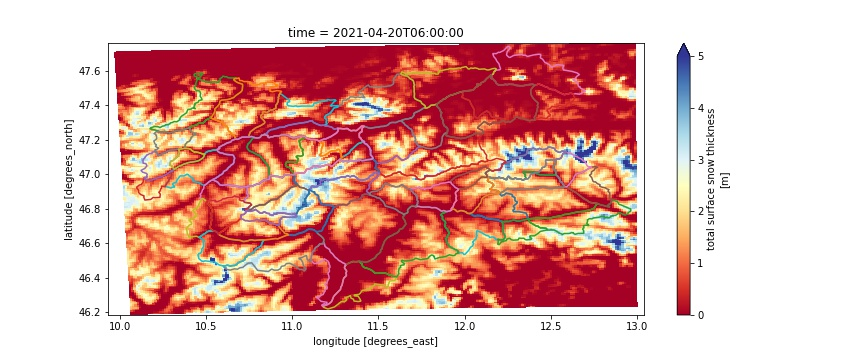
\includegraphics[width=0.8\textwidth]{Figures/figures_methods/snowgrid.jpg}
    \caption{Total snowhight of the SNOWGRID model for the 1st March 2021 06:00:00 MEZ}
    \label{fig:snowgrid}
\end{figure*}

\noindent In order to validate the Regions relevant for avalanche warning service EUREGIO only the wintermonths from Oct till March 
over the periods of the past 10 years (November 2011 till March 2021) comes into account. In the scope of a saveing computing 
power the spatial resolution of 100x100m is reduced to 1x1km by taking the median within this spector. 
Based on the 06:00:00MEZ datastamp a 24h surface hight change will be calulated.

% ==== Cost733cat ===============================================================

\subsection{Cost733cat - Weather and circulation type classification}
\label{sec:wetterlagenkat}
The Cost733cat is a databease of weather and circulation type classfication covering a spatial domain over Europe with 
12 sup domains of the ZAMG. The inputdata comes from ERA40-reanalysis dataset provided by the Eruopian Center of Medium-Range
Weather forecast by \textcite{philippCost733catDatabaseWeather2010}. The domain of intresst of this research is D06 covering
the alps. 

\noindent The Cost733cat contains informations about the main wind direction, cyclonisity and humidity on different pressure levels
weighted to the center of the domain. For these research only the information about the main flow at 700 hPa is of intresst.
The main flow is devided into 9 windsectors, 4 main wind sectors, 4 side wind sectors and one additional class for changing 
wind regimes within a day. For further statistical analyis it has to be taken into account that main sectors has a coverage of
30 $^{\circ}$ and side sectors 60 $^{\circ}$:
\\

\begin{minipage}{.5\linewidth}
    \begin{itemize}
        \item 345$^{\circ}$ -   15$^{\circ}$  \dots   N
        \item 15$^{\circ}$  -   75$^{\circ}$    \dots NE
        \item 75$^{\circ}$  -   105$^{\circ}$    \dots E
        \item 105$^{\circ}$  -   165$^{\circ}$    \dots SE
        \item 165$^{\circ}$  -   195$^{\circ}$    \dots S
        \item 195$^{\circ}$  -   255$^{\circ}$    \dots SW
        \item 255$^{\circ}$  -   285$^{\circ}$    \dots W
        \item 285$^{\circ}$  -   345$^{\circ}$    \dots W
    \end{itemize}
    \end{minipage}
    \hfill
    \begin{minipage}{.5\linewidth}
    \centering
    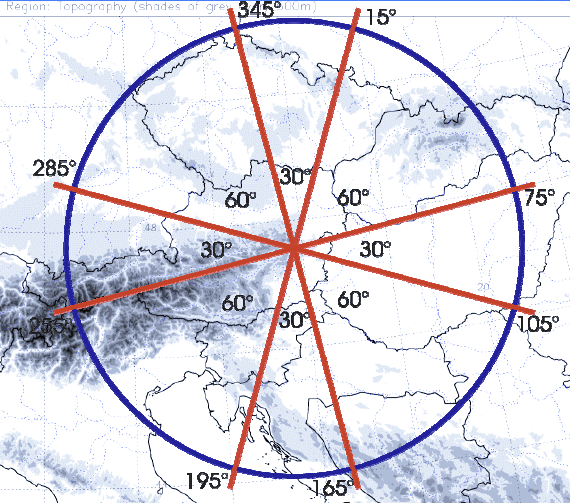
\includegraphics[width=\linewidth]{Figures/figures_methods/windesctors.png}
    \captionof{figure}{Windsectors of the Cost733cat \textcite{krennertWetterlagenklassifikationenZAMGAnfangen}}
    \end{minipage}

% ==== Clustering ===============================================================

\subsection{Clustering}

\noindent The analysis are bases on daily total snow height ($HS$) from the SNOWGRID database of the ZAMG over for the winterseasons
for the area of the EUREGIO, from November 2011 till March 2021. Only days with a percipitation rate from at least 
5mm comes into acount. The initial dataset is based on the INCA grid with a spatial resolution of 100x100m. In the scope of saving computing
time the resolution is reduced to 1000x1000m to the median value of the higher grid. Based on the daily total snowheight
the 24h snowheight change ($delta_{HS}$) is calculated.

\noindent Based on the findings of the Cost733cat the snowgrid datasets are reduced to north blocking situations, south blocking situations 
and all days. For each dataset a k-means algorithm is applied to achive regions with similar percipitation patterns.

\subsubsection*{K-means Clustering}

The k-means clustering method is used to generate groups of vectors $x_j$ with the scope of a small variances of the traget value
within a group. The k-means method is often used to generate similar groups due to its relativly fast computation time. 
On the downside the number of clusters $k$ must be predivend. For $x_j$ datapoints with the 

\begin{equation}
    J =  \parallel x_j -\mu_i \parallel ^{2}
    \label{equ:cluster}
 \end{equation}

 To determin the optimal numbers $k$ of clusters the $ellbow-method$ is drawn by. To do so the sum of the square distance between the points in 
 a cluster are calculated for increasing cluster number k. At the point where a increasing of clusters do not lead to a significantn 
 change the theoretical optimum is reached.  

 \begin{figure*}[h]
    \centering
    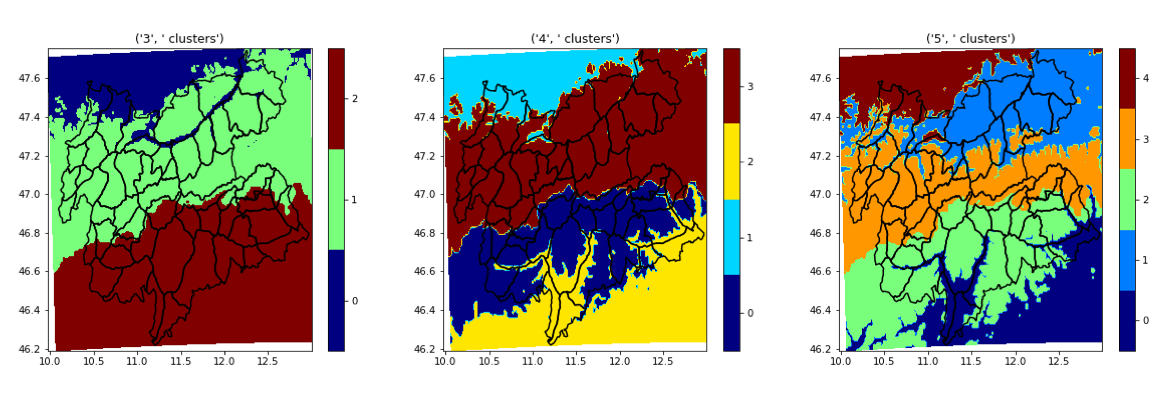
\includegraphics[width=0.8\textwidth]{Figures/figures_methods/number_clusters.png}
    \caption{nr}
    \label{fig:number_of_clusters}
\end{figure*}

To apply the k-means algortihm to our \\
- kmeans\\
- reshaping 3D into 1D \\
- all wind regimes \\
-north blocking \\
- number of clusters \\
 
% ==== Assesing Avlanche Problems ===============================================================
\section{Avalanche classification} 

\subsection{Avalanche types}

Avalanches are as versatile as snow crystals and therefore different types can be determinded based on different critireas
as triggering mechanism, humidity, flow. The most prominant avlanche type critical for snow recrationist are slab avalanches


-Auslöse mechanismus \\
- Lage der Gleitfläche \\
-feuchtigkeit \\
-from-bewegund \\

- dry / wet \\
-slab - loose - gliding - wet snow

- release mechanism \\

- Lawinen --> Brett SCHW ininitianin\\



\subsection{Avalanche Problems}

Due to similar weather phenoms in winters similar snow conditions devlop. The Europian avlanche warning services (EAWS)
agreed in 2018 on five typical avalanche problems describing significant condintions avalanche forcasters and winter sport
enthusiast meet in the back country. They should help in their assessment of the avalanche hazard. Besides the avalanche danger level, the avalanche problem is the 2nd part of the information pyramid
of an avlanche bulletin \cite{mittererAusbildungshandbuchTirolerLawinenkommissionen2022}. Furthermore Avalanche problems
contains information about the expected avalanche type, the distribution, and the location of the weak layer. 

\begin{figure*}[h]
    \centering
    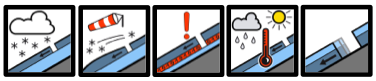
\includegraphics[width=0.8\textwidth]{Figures/figures_methods/avaprobs.png}
    \caption{The five avalanche problems agreed by the EAWS: New snow, Wind slab,Persitent weak layer, Wet snow, Gliding snow}
    \label{fig:avaprobs}
\end{figure*}

% ==== Avalanche Problems ===============================================================
\subsubsection{New snow}

The \textit{New snow}- problem is related to current or most recent snowfall.
Snowfall stand alone does not go hand in hand with a \textit{New snow} problem.
The snowpack has to fullfill curtain critiarias as for example exceeding a critical ammount of snow. 
How critical the loading is depends on various factors such as temperature or characteristics of the old snow surface. 
\cite{mittererAusbildungshandbuchTirolerLawinenkommissionen2022} \\

\noindent In the scope of the \textit{New snow} problem there may accore dry-slab avalanches due to additional load on a old or newly 
build weak layer, or dry-loose snow avalanches in steep terrain due to unsuficient coherence of the snow cristals. 
\\
\noindent The advantage of the \textit{New snow} problem is that it is relativly easy to identivy in the terrain and 
furthermore it is often only relevant during the snowfall and a few days on. Is the most recent snowfall influenced 
by wind it is often combindend with an \textit{Wind Slab}  problem.\cite{mittererAusbildungshandbuchTirolerLawinenkommissionen2022}


\subsubsection{Wind slab}

Wind, to be precise the transported snow the wind plays the key factor. Snow can be carryied during as well as after the snowfall event. 

\noindent The \textit{Wind slab} problem is build if transported snow, building coherent slabs, overlaying weaklayers leading to dry-slab 
avalanches. \textit{Wind slab} can evolve quickly even during the snowfall event. 
Depending on the snowpack evolution and the type of the burried grains (e.g. for loose snow, graupel,...) 
the problem persits from a few days up to months (eg. faceted crystals, surface hoar) converting into persitent problem.

\subsubsection{Persistent weak layers}

The persitent weak layer problem is characterised by a long persitent layer mainly consiting out of faceted crystals
(Faceted crystals, surface hoar, deph hoar) burried by a critical amount of new snow.

Persistend weak layer problems can be spreat over all aspects but persits longer espacially in shaded areas. It is a
insidious prblem and hard to identivy. Only observed snowpit can help to find them. Espected avalanche types a dry-slab avalanches


\subsubsection{Wet snow}

The Wet snow problem is due to the increasing liquide water content in the snowpack leading to a loss of stability.
The increas of the LWC can be due to radiation, liquid presipitation or and increase of temperature. As soon as the LWC 
reaches a critical threshold the stability decreases as long as it reaches stability again after wet-snow-methamorphism

The expected avalanche types ar wet slab and wet loose snow avalanches.

\subsubsection{Gliding snow}

The Gliding snow problem is assciated with a completly gliding of the entire snowpack on the ground. The are hardly 
predictable but  gliding moth anounce might annoucne the problem.


% ==== Avalnche Problem Algorithm ===============================================================
\section{Avalanche Problem Algorithm}

\subsection{Concept}

- Detection/ Tracking\\
- overall deccion tree\\
-Slab \\
-stability critiarias\\
-avalnche problems




\subsection{New Snow}
- new snow ammount \\
- critical ammount \\
- stability critiarias

\subsection{Wind slab}


\subsection{Persistent Weak layer}
- burried FC 
- coherent slab

\subsection{Wet Snow Problem}
\label{sec:methods_wetsnow}
%- LWC 
%-isothermal
The movement of water through the snowpack is complex and depending on the amount of water.
Water is kept between and dominated by capillary forces at low liquide water content ($\theta_w$)(pendular regime).
A further increasment of $\theta_w$ will lead to a gravitational flow (funicular regime). The transision regime
depends on the graintype. Accordingly at a volumetric liquid water content $\theta_{w,v}$ of 3 \% water will drain and
therefore reduce wet snow stability significantly.\autocite{mittererOperationalSupportingTool2013} 

\noindent Mitterer et al. found out the importance of the arrival time of water at the bottom of the snowpack and therefore
introduced the average liquide water content of the entire snowpack normalized by the starting value of transision 
regime(\autocite{mittererOperationalSupportingTool2013}):

 \begin{equation}
    LWC_{index} = \frac{  \overline{ \theta}_{w,v }    } {0.03} 
    \label{equ:LWC}
 \end{equation}

\noindent Where $\overline{ \theta}_{w,v }$ represents the modelled, avarage volumetric water content within the 
entire snowpack. and $0.03$ the start of the regime transsion according to Conway and Reymond \autocite{conwaySnowStabilityRain1993}.
Further more Mitterer et al. presented that the $LWC_{index}$ peformes quite welle to determin periods with high 
wet-snow activity.\autocite{mittererOperationalSupportingTool2013} 

\noindent Conway and Raymond \autocite{conwaySnowStabilityRain1993} defined three different periods for the wet snow
instability:
\begin{itemize}
    \item increase of LWC towards 1, decrease of stability
    \item timing of maximal instability ($LWC_{index}$ = 1)
    \item Return to stability due to ongoing wet-snow meta-morphism ($LWC_{index}$ > 1 for more than 3 days)
\end{itemize}

\noindent The values for $\overline{ \theta}_{w,v }$ will be taken out of \textit{SNOWPACK} simulations for every layer
for each day at defined wet-time period e.g. 15:00 UTC. Out of them the LWC will be calculated and the state of 
isothermal state will be verified.

\subsection{Gliding Snow Problem}

- hard to predict \\
- paper? 

% ==== SNOWPACK ===============================================================
\section{SNOWPACK- model-chains}

\subsection {AWS}
- chain description \\
- input parameter\\


\subsection {Observed profiles}
- chain description\\
- input data\\
- initializing\\
- Hand hardness parameterization\\
- observed profiles\\
- NWPs

\subsubsection{Input parameters}

\subsubsection{Hand hardness parameterization}